\section{Hash Table}
La Hash Table è una struttura di dati che memorizza i dati in modo associativo. In una tabella, i dati sono memorizzati in un formato array, dove ogni valore di dati ha un proprio valore di indice univoco. L'accesso ai dati diventa molto veloce se si conosce l'indice del dato desiderato.\\~\\
In questo modo, diventa una struttura di dati incui le operazioni di inserimento e ricerca sono molto veloci, indipendentemente dalla dimensione dei dati. La Hash Table utilizza un array come supporto di memorizzazione e usa la tecnica dell'Hash per generare un indice in cui un elemento deve essere inserito o da cui deve essere individuato. \\~\\
In particolare, si considera $U$ come insieme (universo) della chiavi, visto come $I = 0,1, \ldots,|U|-1$. La Hash Table $T$ viene vista come array $T[0,...|U|-1]$, in cui un elemento $x$ è inserito in $T[x.key]$.

\begin{center}
    \begin{tabular}{c}
        \\ 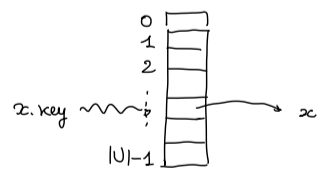
\includegraphics[width=0.4\textwidth]{image/HashTable.png} \\ \\
    \end{tabular}
\end{center}

\paragraph{Problemi:}
\begin{itemize}
    \item Non è possibile avere oggetti con la stessa chiave
    \item OK se il numero $|U|$ è piccolo
\end{itemize}

\begin{mdframed}
\begin{lstlisting}[mathescape=true]
INSERT(T,x)
1   T[x.key] = x        $\Theta(1)$
\end{lstlisting}
\end{mdframed}
\begin{mdframed}
\begin{lstlisting}[mathescape=true]
DELETE(T,x)
1   T[x.key] = NULL     $\Theta(1)$
\end{lstlisting}
\end{mdframed}
\begin{mdframed}
    \begin{lstlisting}[mathescape=true]
SEARCH(k)
1   return T[k]         $\Theta(1)$
\end{lstlisting}
\end{mdframed}
